\documentclass{beamer}
\usetheme{metropolis}           % Use metropolis theme
\title{Primera exposición}
\date{Viernes 30 de julio de 2021}
\author{Jorge Alejandro Rodríguez Aldana}
\institute{Escuela de Ciencias Físicas y Matemáticas}

\usepackage{physics}
\usepackage[spanish]{babel}


\begin{document}
  \maketitle
  \section{Desplazamiento axial de un objeto proyectado por una lente}
  \begin{frame}{Problema 6:}
    % An object is located at a distance U to the left of a
    % thin lens and its image is formed a distance V to the
    % left of the same lens (see Figure II.15). If now the
    % object is displaced axially a small distance dU to the
    % left, find an expression for the corresponding dis-
    % placement dV of the image; dVldU is called the long-
    % itudinal magnification. Show that it is the square of
    % the lateral magnification.

    Un objeto es ubicado a una distancia $U$ a la izquierda de una
    lente delgada, y su imagen es formada a una distancia $V$ a la
    izquierda del mismo lente. Si ahora el 
    objeto se desplaza axialmente una pequeña distancia $\dd U$ a la
    izquierda, halle la expresión para el desplazamiento correspondiente
    $\dd V$ de la imagen. $\dv{V}{U}$ es llamada "magnificación longitudinal". 
    Muestre que esta es igual al cuadrado de la magnificación lateral.

    \begin{figure}
        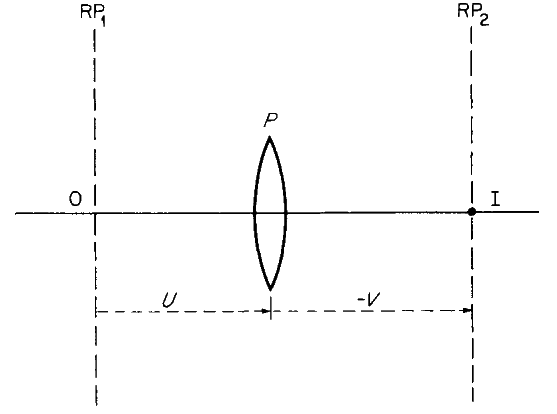
\includegraphics[width=0.3\textwidth]{Figures/Book3.png}
        \caption{Problema 6}
        \label{fig-1}
    \end{figure}
  \end{frame}

  \begin{frame}{Problema 6:}
    \begin{figure}
      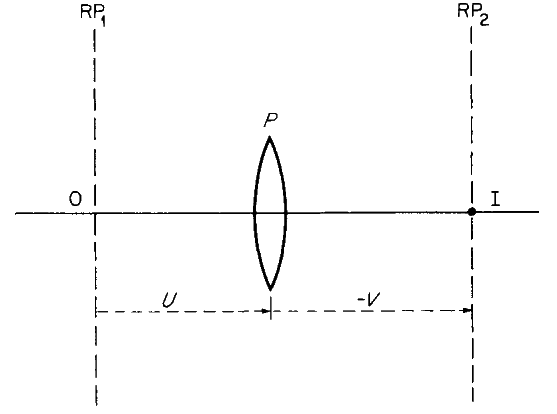
\includegraphics[width=0.5\textwidth]{Figures/Book3.png}
      \caption{Problema 6}
      \label{fig-2}
    \end{figure}
  \end{frame}

  \begin{frame}{Matrices:}
    
    \begin{equation}
      \begin{pmatrix}
        1 & U\\
        0 & 1
      \end{pmatrix}
    \end{equation}
    \begin{equation}
      \begin{pmatrix}
        1 & 0\\
        -P & 1
      \end{pmatrix}
    \end{equation}
    \begin{equation}
      \begin{pmatrix}
        1 & -V\\
        0 & 1
      \end{pmatrix}
    \end{equation}
  
  \end{frame}

  \begin{frame}{Matriz del sistema}
  
    \begin{equation*}
      \begin{pmatrix}
        1 & -V\\
        0 & 1
      \end{pmatrix}
      \begin{pmatrix}
        1 & 0\\
        -P & 1
      \end{pmatrix}
      \begin{pmatrix}
        1 & U\\
        0 & 1
      \end{pmatrix}=
      \begin{pmatrix}
        1+PV & U-V+PUV\\
        -P & 1-PU
      \end{pmatrix}
    \end{equation*}
  
  \end{frame}

  \begin{frame}{Buscamos el punto donde está su imagen}
  
    El elemento $U-V+PUV$ debe ser igual a cero

    \begin{figure}
      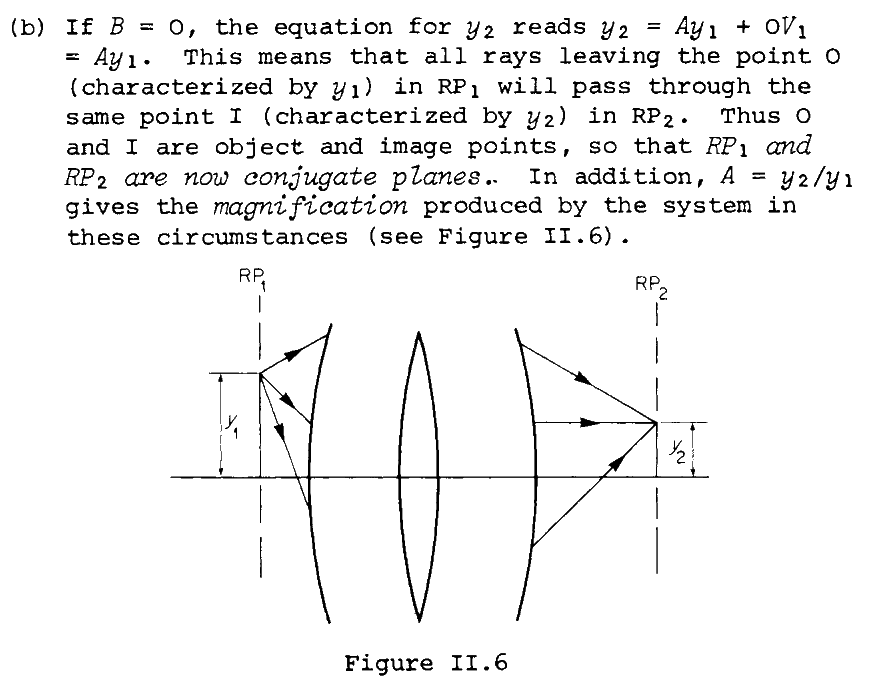
\includegraphics[width=0.6\textwidth]{Figures/B0.png}
      \caption{Explicación de por que este término se anula}
    \end{figure}
  
  \end{frame}

  \begin{frame}{Un poco de álgebra}
  
    Entonces con un poco de álgebra despejamos $V$:

    \begin{align*}
      U-V+PUV&=0\\
      V=\frac{U}{1-PU}
    \end{align*}

    Y derivando:

    \begin{equation}
      \dv{V}{U}=\frac{1}{(1-PU)^2}
    \end{equation}
  
    \begin{equation}
      \dd V=\frac{\dd U}{(1-PU)^2}
    \end{equation}

  \end{frame}

  \begin{frame}{Tabla de referencia}
  
    \begin{figure}
      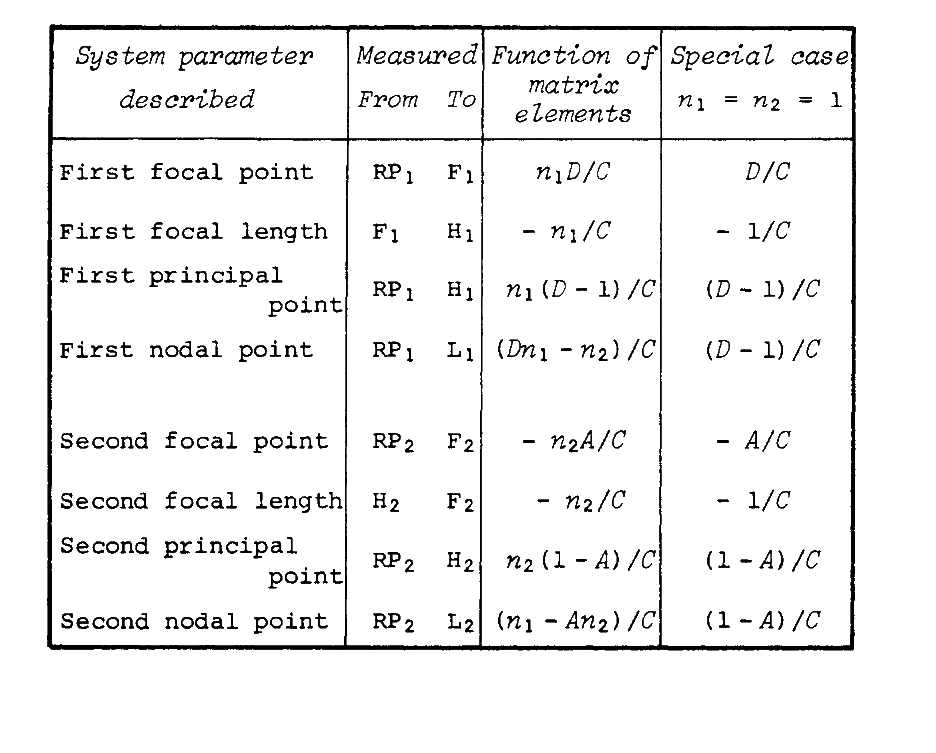
\includegraphics[width=0.8\textwidth]{Figures/TableBook.png}
      \caption{Tabla de referencia tomada del libro}
      \label{fig:Ref}
    \end{figure}
  
  \end{frame}
  

\end{document}

